\chapter{实验原型实现}
根据上面的调研结果,可以改进的方面有很多。但是从用户日常使用的角度,影响用户持续使用最大的问题是可用性的问题和理解的问题。

可用性的解决方案主要分为两块:一个是提高系统的可用性;另一个是重新设计用户友好的交互界面,提升交互的体验。增强用户理解则是通过加入透明性。

\section{设计理念}

在这个平台做透明性的研究,通用实验平台的设计和搭建
日志管理,为了实验,
开关控制,

为什么只用它的这个?

为了支持后续的交互研究,该平台需要提供一下几种特性或者功能:

1. 模型管理

新的人脸相关的模型,能够快速接入系统。当前人工智能发展迅速,不断有新的模型出现,为了让新的模型能够快速接入,系统需要对模型进行抽象,能够快速将模型应用到系统,以便开展实验工作。

2. 日志管理

分析及最终用户的行为。

3. 问卷关联

可定制的话问卷可以完成个人信息采集,资格测验,前后对比等功能。

4. 快速迭代

客户端最好能快速获取到最新的版本。

\section{跨平台系统设计}
\subsection{技术探针系统设计}
作为我们技术探针的云中医只有Android版本,核心诊断和打分算法使用c++编写, 分类模型为OpenCV模型。
在具体实现方面,将所有OpenCV格式模型打包到Android安装包中,在Android平台通过Native方法调用动态链接库的方式完成诊断。

这种非跨平台的实现,有一个明显的缺点就是系统的稳定性需要考虑的用户各种设备环境。在用户调研过程中,很多用户曾经反馈在使用过程中无法完成诊断或者闪退。

\subsection{新系统设计}
解决跨平台需要同时实现IOS,Android,以及Web平台应用,目前云中医已经有安卓版本的实现,模型调用是通过Java调用Native动态链接库的方式。
在实现IOS和Web平台应用时,经过考虑有以下方案:

\subsubsection{方案一}
 IOS重新编写一套代码,通过swift语言调用链接库的方式调用模型; Web平台重新编写一套代码,通过接口调用的方式调用模型。

优点: Android 平台核心代码不需要改动,只需要修改交互和界面。模型文件放在客户端,有安全风险。

缺点: 需要重新编写IOS和Web平台代码,需要同时维护三个平台的代码,保持功能界面的一致性。移动端平台模型是本地调用,不方便统一管理。模型本地调用需要考虑客户端的系统平台和设备性能。

\subsubsection{方案二}
采用C/S架构,全部重写。IOS,Android以及Web客户端使用一套H5代码, 处理逻辑在服务端实现,模型独立服务化,通过Http接口的方式调用。

优点: 客户端使用一套H5代码,维护方便。模型部署在服务器,无泄密风险,可以统一管理(统计调用次数,记录错误日志等),方便实现高可用。

缺点: 依赖网络稳定性,重写的工作量稍大, 需要另外实现模型服务化和服务端。

方案一的缺点会导致后续的维护成本过大,本文最终采用方案二。

如图\ref{fig:system}所示,系统主要分为三部分:服务端和客户端,算法模型通过容器的方式服务化成模型池。

\begin{figure}[ht]
    \centering
    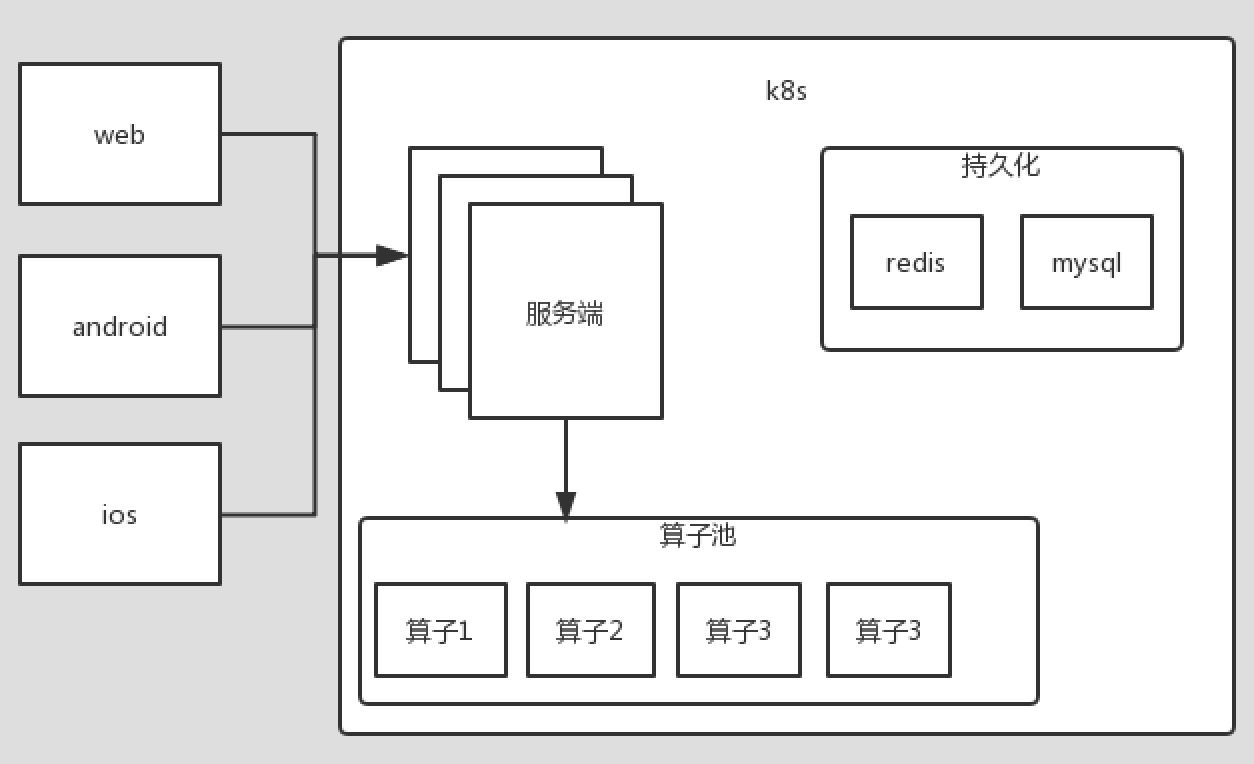
\includegraphics[width=12cm]{images/system.png}
    \caption{跨平台系统设计}
    \label{fig:system}
\end{figure}

一次诊断的大致流程如下:用户通过客户端,上传图片或者回答问题,客户端则向服务端发起请求。服务端收到请求之后,进行任务分配,对分配到任务的实例,调用模型池中对应的模型完成特征提取或诊断打分,同时将数据持久化到mysql和磁盘中,然后把结果返回给客户端。客户端收到服务端的结果后,根据用户是否透明,进行结果的展示。

\section{模型池}

模型池由多个独立可用的模型服务构成, 通过http 接口调用完成和服务端的交互进行任务处理。

首先,通过Flask框架建立一个Http的服务,把特征提取模型打包成服务。每个特征提取服务,可以接受http的请求,对传过来的图片进行特征提取。
模型的计算能力如 表\ref{tab:face-feature}, 表\ref{tab:tongue-feature}, 表\ref{tab:diag-feature}所示。

云中医目前现有两类可用的模型,特征提取模型(面部和舌部两种)和诊断打分模型,分别有对图片进行特征提取和对特征进行打分的能力。
其中特征提取模型只返回了最终结果,诊断打分模型暴露了一部分中间结果。

\begin{table}[]
    \centering
    \begin{tabular}{lll}
        \toprule
        特征          & 特征描述     & 特征内容 \\ 
        \midrule
        faceDetectRes & 人脸   & 0:未检测出人脸,1:成功检测出人脸  \\
        faceColor     & 面部颜色 & 0:面白,1:面黑,2:面红,3:面黄,4:面青,5:正常 \\
        faceGloss     & 面部光泽 & 0:有光泽,1:少光泽,2:无光泽\\
        lipDetectRes  & 嘴唇   & 0:未检测出嘴唇,1:成功检测出嘴唇\\
        lipColor      & 嘴唇颜色 & 0:淡白,1:淡红,2:红,3:暗红,4:紫   \\
        \bottomrule
    \end{tabular}
    \caption{脸部特征提取模型输出}
    \label{tab:face-feature}
\end{table}

\subsection{脸部特征提取模型}
如表 \ref{tab:face-feature} 所示,脸部特征提取模型,输入为面部特征图片,输出有以下几个维度:

1. 是否检测到人脸(faceDetectRes):如果没有检测到人脸,则剩余所有维度无效,且取值为0。

2. 是否检测到嘴唇(lipDetectRes): 如果没有检测到嘴唇,嘴唇颜色的结果无效且取值必定为0。

3. 面部颜色、面部光泽(faceColor、faceGloss) : 面色和光泽是对预处理之后的图片,去除眼口鼻区域的图片进行面色和光泽信息提取的结果。

4. 嘴唇颜色(lipColor): 嘴唇颜色的结果从浅到深分别为淡白,淡红,红,暗红,紫。

\begin{table}[]
    \centering
    \begin{tabular}{lll}
        \toprule
        特征 & 特征描述 & 特征内容 \\ 
        \midrule
        tongueDetectRes & 舌体 & 0:未检测出舌像,1:成功检测出舌像 \\
        tongueCrack & 舌裂纹 & 0:未检测到裂纹,1:成功检测到裂纹 \\ 
        tongueFatThin & 舌胖瘦 & 0:正常(瘦),1:胖舌 \\
        tongueCoatThickness & 舌苔厚薄 & 0:薄,1:厚 \\
        tongueCoatColor & 舌苔颜色 & 0:苔白,1:苔黄 \\
        tongueNatureColor & 舌质颜色 & 0:舌暗红,1:舌淡白,2:舌淡红,3:舌红,4:舌紫\\
        \bottomrule
    \end{tabular}

    \caption{舌部特征提取模型输出}
    \label{tab:tongue-feature}
\end{table}

\subsection{舌部特征提取模型}
如 表 \ref{tab:tongue-feature} 所示,舌部特征提取模型,输入为舌头图片,输入有以下几个维度:

1. 是否检测到舌体(tongueDetectRes): 如果没有检测到舌体,则剩余所有维度无效,且取值为0。

2. 是否检测到舌裂纹(tongueCrack): 舌裂纹是最终特征,剩余特征是否有效和该标志位没有关系。

3. 舌头特征(tongueFatThin、tongueCoatThickness、tongueCoatColor、tongueNatureColor): 包括舌胖瘦,舌苔的厚薄,颜色和舌质颜色。

\begin{table}[]
    \begin{center}
        \begin{tabular}{lll}
            \toprule
            特征 & 特征描述 & 特征内容 \\ 
            \midrule
            healthScore & 健康分数 & 0-100 \\
            healthType & 是否包含某种体质 & {[}0, 0, 0, 0, 0, 0, 0{]} \\ 
            questionScore & 各种问题的体质得分 & {[}0, 0, 0, 0, 0, 0, 0{]} \\
            symCount & 各种体质症状个数 & {[}0, 0, 0, 0, 0, 0, 0{]} \\
            symNum & 总体体质症状个数 & 0-13 \\
            baseScore & 基本分数 & 0-100 \\
            phy & 体质结果 & 八种体质中的一种\\
            \bottomrule
        \end{tabular}
    \end{center}
    \caption{诊断打分模型输出}
    \label{tab:diag-feature}
\end{table}

\subsection{诊断打分模型}
原版的云中医应用中,只给用户暴露了健康分数和体质结果。
如表 \ref{tab:diag-feature} 所示,最终诊断打分模型的体质结果输出为 "阳虚","阴虚", "痰湿","瘀滞", "脾虚", "肾虚", "气虚", "健康" 中的一种,具体的特征说明如下:

1. 健康分数(healthScore): 打分的最终健康分数,由baseScore、symNum、questionScore计算而来。

2. 体质类型(healthType): 大小为7的数组,对应 "阳虚","阴虚", "痰湿","瘀滞", "脾虚", "肾虚", "气虚", "健康"。如果包含某个体质,对应位置的值为1。

3. 问题得分(questionScore): 一共有13个问题,每个问题都会影响最终体质的倾向得分, questionScore是所有问题的得分的累加。

4. 症状个数(symCount): 13个问诊问题中,对应有某个体质特征的症状的累加。

5. 总体症状个数(symNum): symCount的求和。

6. 基本分数(baseScore): 打分模型中, healthScore=baseScore*p + 症状分数*q ,对应不同的症状个数,计算最终得分用的baseScore是不一样的。 
p和q是模型中预设的权重, 症状分数由问题得分计算而来。

7. 体质结果(phy): 和healthType对应,给出用户的体质倾向。



模型服务使用docker进行打包,通过k8s管理多个模型高实现可用。服务端通过k8s提供的集群 ip进行调用。
为了减少读写的竞争,模型池中的服务只进行计算,不进行mysql和redis的读写,结果的持久化由服务端完成。

\section{服务端}

服务端使用Django框架实现,允许有多个实例同时运行,共同处理用户发起的诊断任务,使用redis和mysql进行数据的持久化。
Redis是基于内存的分布式数据库,在本系统中主要保存服务端可用节点的信息。
Mysql是当前比较流行一个关系型的数据库,在本系统主要主要保存日志信息,任务信息等。

服务端的主要模块如图 \ref{fig:server} 所示, 其中日志管理提供了网页端的管理界面,能够在线地对日志进行查询导出;任务管理为客户端提供了任务提交和结果查询接口,为客户端的面诊、舌诊、问诊提供支持。
系统通过设置定时器,定期地发送心跳包进行主从竞选,主节点会进行人物分配,主节点和从节点则对分配到的人物进行执行,调用模型池中对应的模型完成任务。


\begin{figure}[ht]
    \centering
    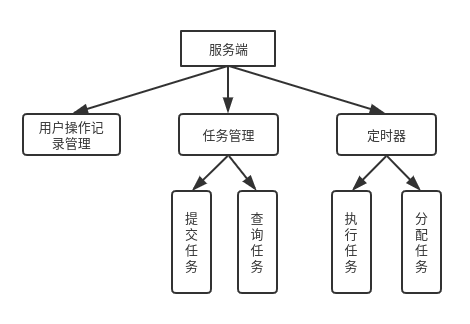
\includegraphics[width=12cm]{images/server.png}
    \caption{服务端主要模块设计}
    \label{fig:server}
\end{figure}


\subsection{日志管理}
为了方便后续的数据分析,我们需要采用用户的所有操作日志。日志的数据库主要字段如表 \ref{tab:op_log} 所示:

\begin{table}[]
    \centering
    \begin{tabular}{lll}
        \toprule
        字段 & 类型 & 描述 \\ 
        \midrule
        id & int & 主键 \\
        user, & text & 用户唯一标识 \\ 
        device & text & 所用设备信息 \\
        op & text & 操作名 \\
        info & text & 操作信息 \\
        createTime & datetime & 创建时间 \\
        updateTime & datetime & 更新时间\\
        \bottomrule
    \end{tabular}
    \caption{操作日志表}
    \label{tab:op_log}
\end{table}


其中,user字段用于标识用户,默认使用用户手机号作为唯一标识,要求用户进入系统前需要通过手机验证码进行登录。而在后续的透明性实验环节,为了方便用户跳转完成问卷,不需要用户进行登录,user字段采用的是wjx-问卷星id。

\begin{figure}[ht]
    \centering
    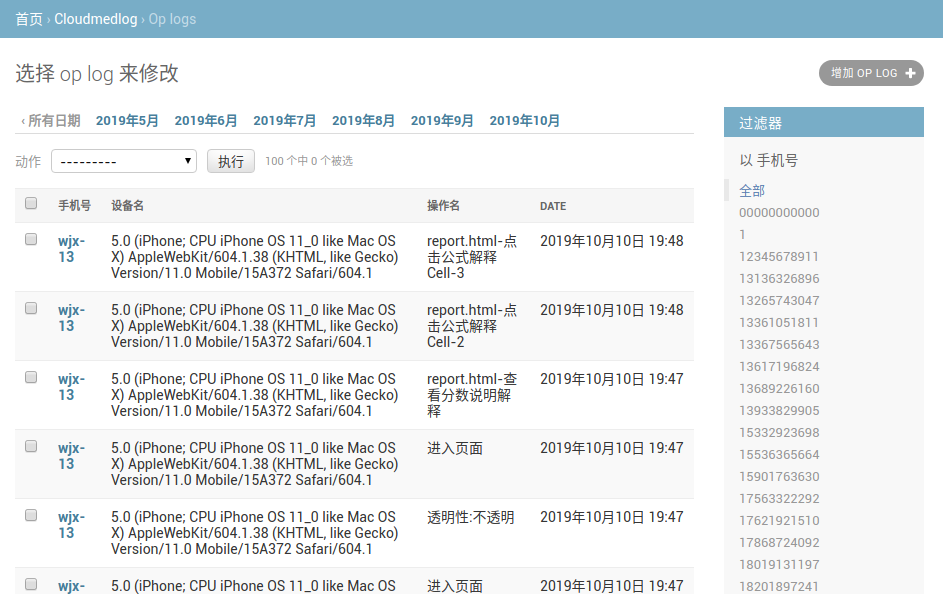
\includegraphics[width=15cm]{images/op_log.png}
    \caption{日志管理界面}
    \label{fig:op_log}
\end{figure}

\subsection{任务处理}
一次用户诊断,服务端需要完成多个任务:面部特征提取任务,舌部特征提取任务,问诊打分任务。
服务端在收到用户提交的任务之后,会将数据存储到数据库的task表中,task表的主要字段如表 \ref{tab:task}所示:

1. type一共有四种取值,目前对应四种任务类型:面部特征提取任务,舌部特征提取任务,诊断任务和合并任务。

2. in为任务的输入,其中面部特征提取和舌部特征提取任务需要的输入为图片,通过Base64编码序列化为json对象,保存在in字段中。

3. out为任务的执行结果,在模型池的服务完成计算之后,服务端将任务执行结果保存到out字段,同时更新任务的状态。

4. handler保存当前任务是由哪个服务端在负责处理。

5. extra通过json格式存储模型相关信息,如分类任务,如体质判别,输出的7中体质的中文名称,保存在extra中。

\begin{table}[]
    \centering
    \begin{tabular}{lll}
        \toprule
        字段 & 类型 & 描述 \\ 
        \midrule
        id & int & 主键 \\
        type, & int & 任务类型: 面部,舌部,诊断, 合并 \\ 
        extra & json & 模型相关信息 \\
        in & text & 任务输入 \\
        out & text & 任务结果 \\
        handler & text & 分配的服务端 \\
        status & int & 任务状态: 新建,已分配,处理中,失败,完成 \\
        createTime & datetime & 创建时间 \\
        updateTime & datetime & 更新时间\\
        \bottomrule
    \end{tabular}
    \caption{任务表}
    \label{tab:task}
\end{table}

\subsection{任务分配}
为了实现服务的稳定性,服务端支持同时开启多个实例,即多个服务端同时处理任务。
同时考虑到性能,服务端设计为读写分离的架构:每个实例都可以读取任务列表,处理用户的任务,但只有主节点有任务分配的权限。

服务端通过心跳包探活,主节点失效时,通过redis的分布式锁实现主节点的竞选。


\subsubsection{主从节点的职责}

1. 主节点: 通过任务的id进行哈希,按照哈希进行任务的分配给各个节点,更新task表。

2. 从节点: 每个从节点每过一定的间隔时间,就会去读取任务列表,开始执行任务列表里属于自己的任务。

\subsubsection{服务端角色竞选流程}
\begin{figure}
    \centering
    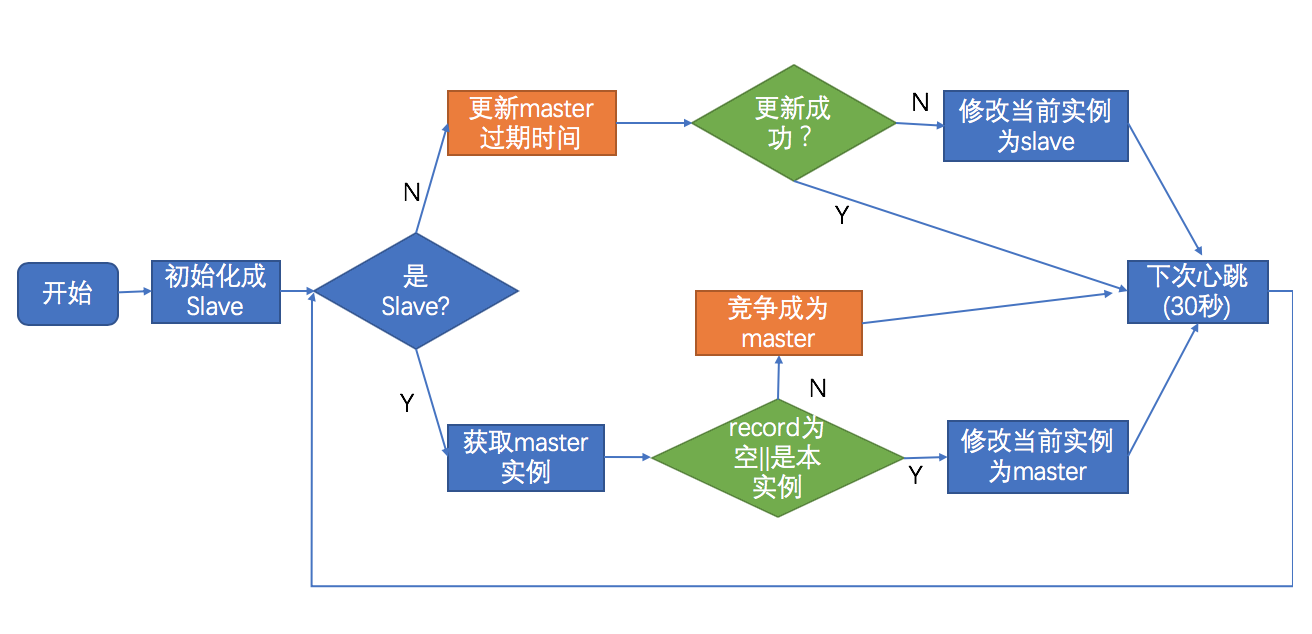
\includegraphics[width=10cm]{images/slave-master.png}
    \caption{服务端角色竞选}
    \label{fig:slave_master}
\end{figure}
每个节点在启动之后,会在本地把自己的角色默认设置成从节点。

然后每过一段时间,判断自己节点的类型,主从节点分别执行以下的心跳策略:

主节点:主节点每次心跳的时候,更新redis中主节点的过期时间。如果更新成功,等待下一次心跳; 
如果更新失败(更新失败可能是自己没有及时更新,导致redis里的主节点过期,主节点的身份被其他节点竞争到了),则把自己的节点类型设置成从节点。

从节点:从节点每次从redis里获取主节点的信息,如果主节点信息无效或者长时间没有心跳(默认设置为两轮心跳周期),则开始抢占竞选锁,尝试更新redis的信息让自己成为主节点;
如果redis的主节点信息已经是本节点,说明上一轮抢占成功,将本节点的角色更新为主节点。

\subsection{结果合并子任务}
合并任务只有前置任务,没有后置任务,它是整个任务调度流程中的最后一个任务。合并任务的主要功能是在所有计算类型的任务完成后,对计算出来的结果进行合并。

合并任务的触发时机,是在合并任务的所有前置任务完成之后。合并任务的合并流程如下:



\section{客户端}
IOS, Android和Web平台客户端都采用同一套代码,采用MUI+AngularJS实现。
MUI是一个高性能前端框架,本身不依赖任何的第三方JavaScript库,实现了接近原生的用户体验,并内置了大量组件。
AngularJS目前是Google公司的JavaScript框架,支持快速构建移动应用。

客户端的主要工作,是设计新的自诊界面,解决交互方面大量易用性的问题。整体的设计思想是给用户对自己当前状态一种直观的感受。

客户端系统主要有以下几个部分:用户登录,健康诊断(面诊,舌诊,问诊),健康报告,诊断记录。

\subsubsection{用户登录}
\begin{figure}[ht]
    \centering
    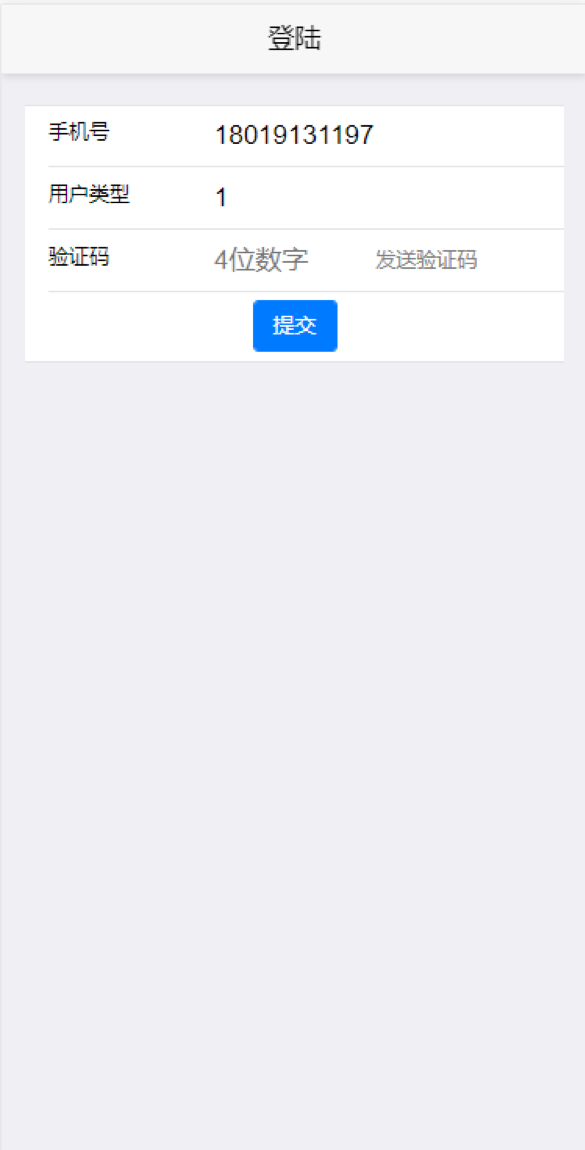
\includegraphics[height=5cm]{images/login.png}
    \caption{用户登录}
    \label{fig:login}
\end{figure} 
用户登录时,需要输入正确的手机号才能通过手机格式验证发送验证码到手机上。登录界面可以接受一个ssojump的参数,用于判断是否来自问卷星。如果验证通过,则直接跳过登录进入首页。
在用户登录时,用户可以看到自己的用户类型:1代表不透明模式,2代表透明模式。
透明模式和不透明模式是本系统设计的两种用户类型,在透明模式下,用户可以看到所有的面诊,舌诊,问诊的中间结果和对最终结果的影响,同时也对相关的概念呢和依据进行了详细的解释。
系统是如何实现透明模式的会在后续详细进行解释。

\subsubsection{健康诊断}

\begin{figure}[h]
    \centering
    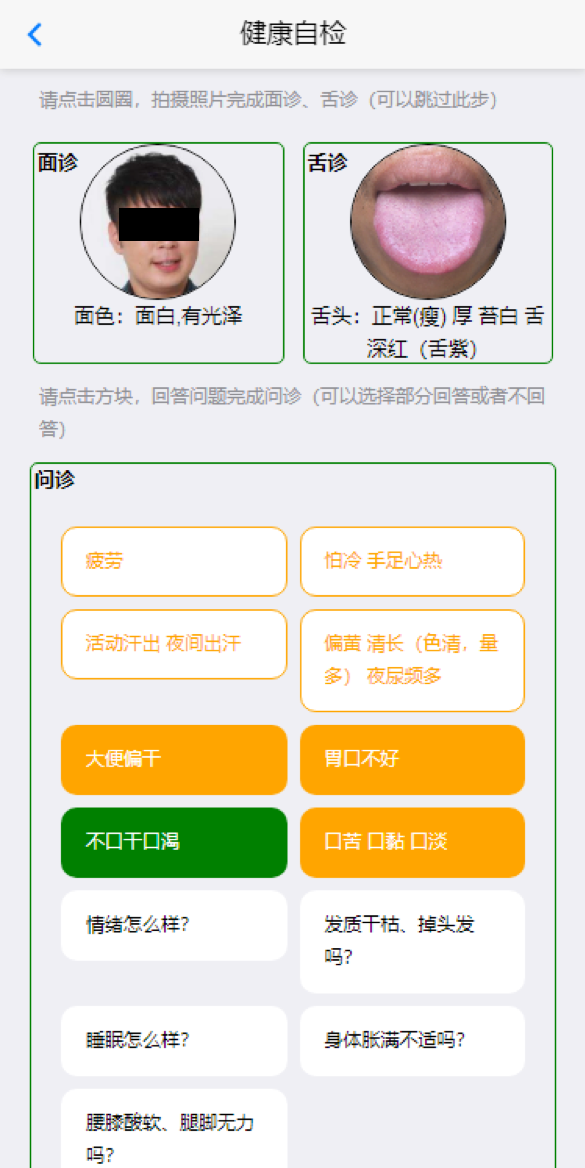
\includegraphics[height=10cm]{images/diag.png}
    \caption{面诊舌诊问诊新界面}
    \label{fig:diag_new}
\end{figure}
在原始的云中医版本中,用户在进行面部舌部拍照后,是没有任何提示的。具体的结果需要在用户一次回答13个问题之后,点击诊断才能知道面诊是否成功。
新界面和之前版本的云中医界面不同的是,诊断界面不仅提供了面诊舌诊问诊的入口,同时会将面诊舌诊的照片和中间结果直接显示在当前页面,给用户对于自己当前身体情况一个直观的感受。
如果拍照失败会直接显示,不需要等到用户进行点击诊断之后才知道自己的照片不合格。
    
如图\ref{fig:diag_new}所示,根据用户调研的反馈,新界面简化了诊断的流程,面诊舌诊问诊在一个页面显示,并且所有的问题和操作都是可选的,不会出现必须要先面诊然后舌诊然后才能问诊的问题。其次,新界面对面诊和舌诊进行了中间结果的反馈,面诊在用户拍照确认之后,会立即报告本次照片是否合格已经诊断的结果,用户不需要在点击诊断的时候才被提示照片不合格。

在问诊方面,新系统实现了最近一次记录保存,由于问题是可选回答的,所以用户只需要回答和自己上次的结果不一致的即可。同时,我们对不同问题的回答结果进行了颜色的区分。有色实心代表本次回答,有色空心代表上次回答;橙色代表有症状,绿色代表回答的问题表现良好,没有症状;白色没有填充和边框,为黑字,代表未回答。

在方框内部的问题描述设计上,如图 \ref{fig:diag_new} 所示,我们把默认的文字描述,显示为问题描述;一旦用户本次或者上次回答过该问题,则直接显示用户回答的结果。这样做的结果是,第二次用户点进来,就能看到上次的回答结果,这样能够对自己的身体情况有个快速的了解。

% \subsubsection{照片上传}

\begin{figure}
    \centering
    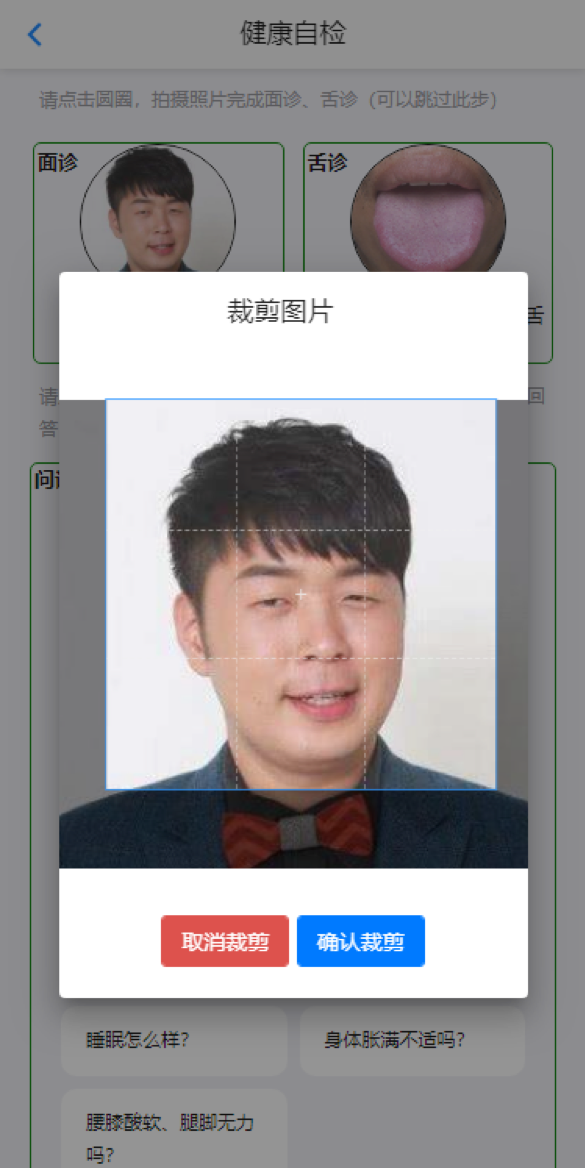
\includegraphics[height=10cm]{images/crop.png}
    \caption{图片裁剪}
    \label{fig:crop}
\end{figure}
% 用户通过点击面诊或者舌诊的圆圈图案,可以通过从相册选择或者通过拍照,上传自己的脸部或者舌头照片。
% 图片裁剪可以帮助用户定位面部和舌头的位置,提高诊断的精度。用户点击确认裁剪之后,诊断的结果会直接显示在圆圈下面,同时,如果没有识别到人脸或者舌头也会提示用户重新拍照。
% 点击确认裁剪后,通过对图片进行base64编码上传到服务器的诊断接口,服务器调用模型池对应模型,拿到诊断结果。

\subsubsection{问诊}

\begin{figure}
    \centering
    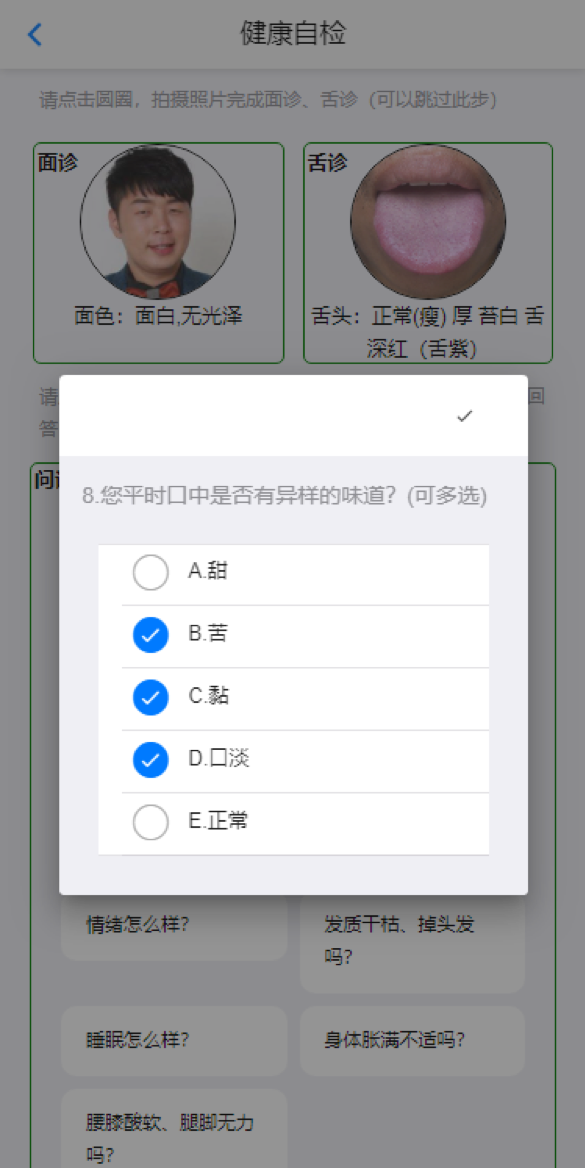
\includegraphics[height=10cm]{images/questions.png}
    \caption{问诊}
    \label{fig:questions}
\end{figure}
问诊的问题一共13道,用户根据自己的情况通过勾选回答问题。每次进入问诊界面,系统会尝试加载上一次用户回答问题的历史记录和对应的答案。
同时,回答过的问题,会在界面上进行显示。没有回答过的问题,将是白色黑字没有边框。

用户在完成自己需要回答的问题或者面诊舌诊之后,可以点击蓝色的诊断按钮进行健康诊断,同时,系统会将本地诊断记录上传到后台服务器上,以便查询诊断记录。

% \subsubsection{诊断结果}
% \begin{figure}[ht]
%     \centering
%     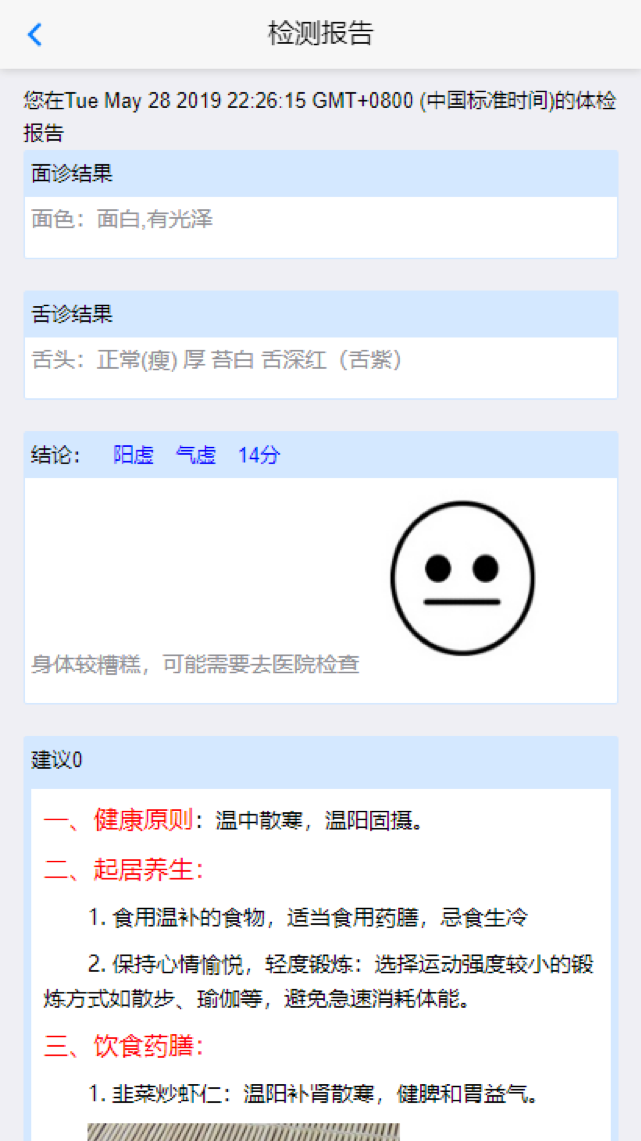
\includegraphics[height=10cm]{images/report.png}
%     \caption{健康报告}
%     \label{fig:report}
% \end{figure}
系统根据用户个人的情况,会给出面诊结果,舌诊结果和最后的体质以及健康分数。此外,根据体质的不同,会给出和体质对应的健康建议,帮助用户进行针对性的健康调理。

\subsubsection{诊断记录列表}
\begin{figure}[ht]
    \centering
    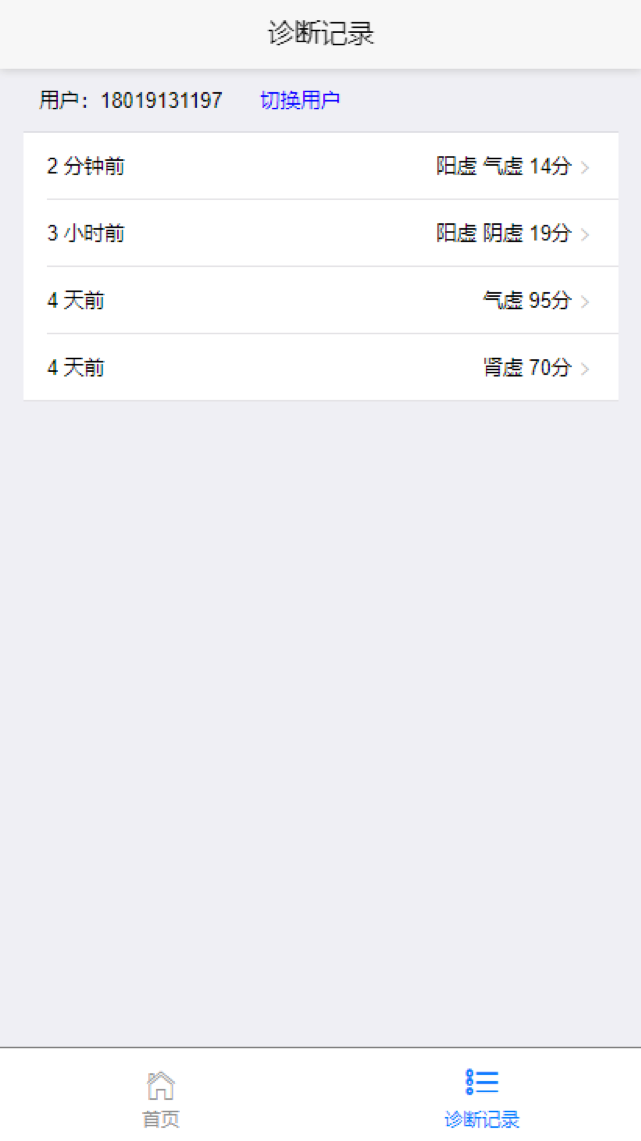
\includegraphics[height=10cm]{images/history.png}
    \caption{诊断历史}
    \label{fig:history}
\end{figure}
诊断记录页面,能够直观地给出用户近期的健康变化的情况。用户可以点击诊断记录,进入当时的详细诊断结果页面。

%%%%%%%%%%%%%%%%%%%%%%%%%%%%%%%%%%%%%
\section{系统可解释性}

已有大量的研究表明,增加系统的可解释性,是可以提高用户对系统的信任程度的。
考虑到中医应用的特殊性,普通用户需要提高对应用的理解。因此我们在系统中加入算法的解释性,提升用户的体验。而根据之前的用户调研来看,由于当前诊断和打分模型存在改进的空间,部分的用户也对结果产生了怀疑或者对结果不理解。
在这个基础上,我们希望通过讲模型的判决过程透明化,并对结果进行解释。

在具体代码实现的时候,系统对于是否过程透明、对结果进行解释是通过用户的类型来进行判断的。

对于每一个用户,我们通过哈希算法,对用户名计算哈希值,按照哈希值的奇偶性,将奇数用户归类为不透明用户,偶数用户归类为透明用户。
两类用户在进行面诊舌诊时的流程一样,但是透明用户能够看到背后特征提取算法和诊断算法的中间数据,同时系统为给出的诊断结果进行了解释。


透明性在呈现的时候,大致可以分为两种:

1. 结果中文字结果是有提示可以进行点击。如果用户点击了健康报告的分数,会通过弹窗进行详细的解释。

2. 通过雷达图的方式直接显示对结果的影响,交互性比较强。

\subsection{面诊舌诊过程的解释性}

\begin{figure}
    \centering
    \subfigure[不解释]{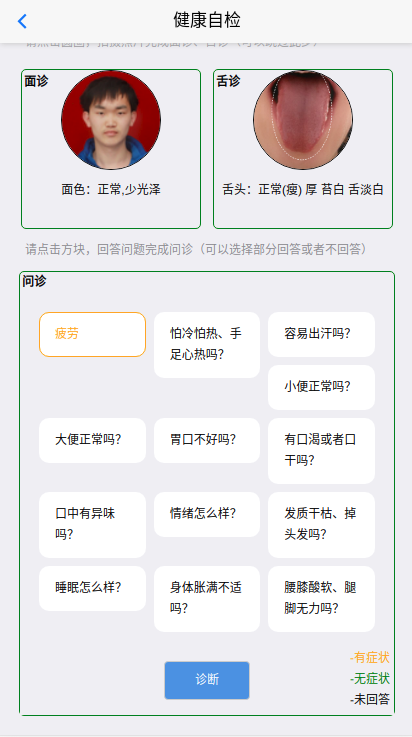
\includegraphics[width=4.5cm]{images/face_tongue.png}}
    \subfigure[解释]{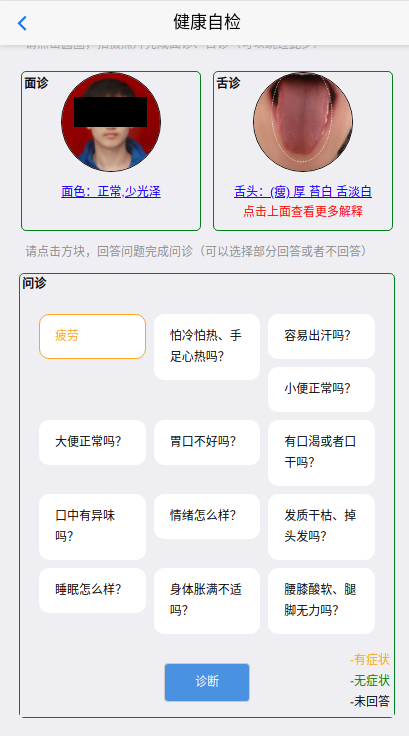
\includegraphics[width=4.5cm]{images/exp_face_tongue.png}}
    \subfigure[解释舌诊中间结果]{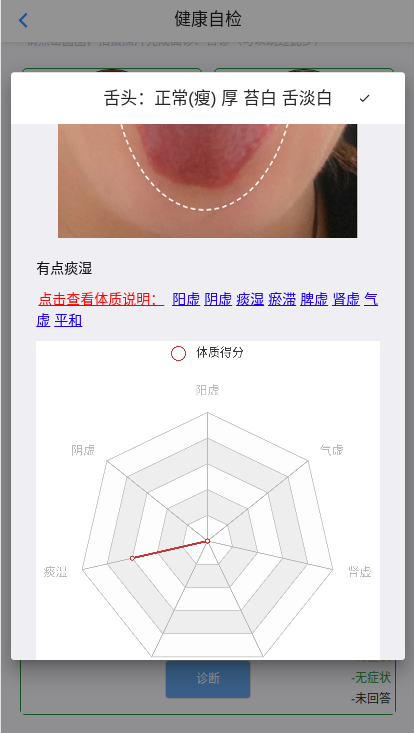
\includegraphics[width=4.5cm]{images/exp_tongue.png}}
    \caption{面诊舌诊的解释}
    \label{fig:face_diags}
\end{figure}

面诊和舌诊流程比较类似,添加透明性主要体现在结果的透明性,包括中间结果,和对各种体质倾向的影响。
这样用户查看解释之后,能够大致了解本次拍照是否成功,并且知道目前面诊的结果,会对最终的健康报告造成哪些影响。

如图 \ref{fig:face_diags} 所示:

a) 普通用户只能看到结果。

b) 透明类型的用户,可以通过点击结果,查看对结果的解释。

c) 透明类型的用户,不仅可以看到当面诊断的中间结果,也能看到这次诊断的体质倾向得分。



\subsection{问诊的透明性}

\begin{figure}
    \centering
    \subfigure[不解释]{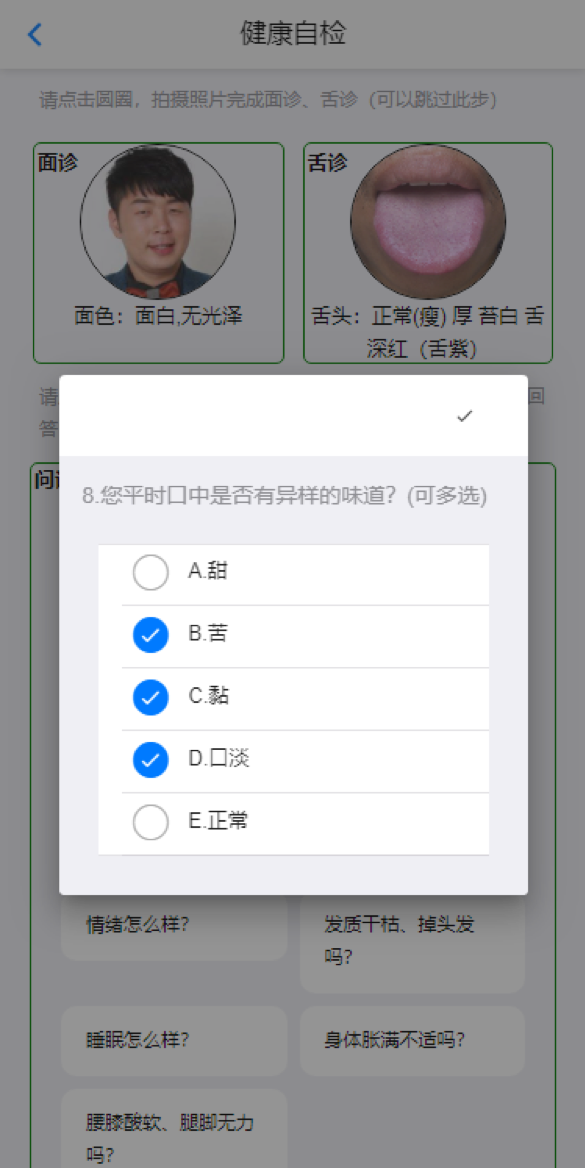
\includegraphics[height=10cm]{images/questions.png}}
    \subfigure[解释]{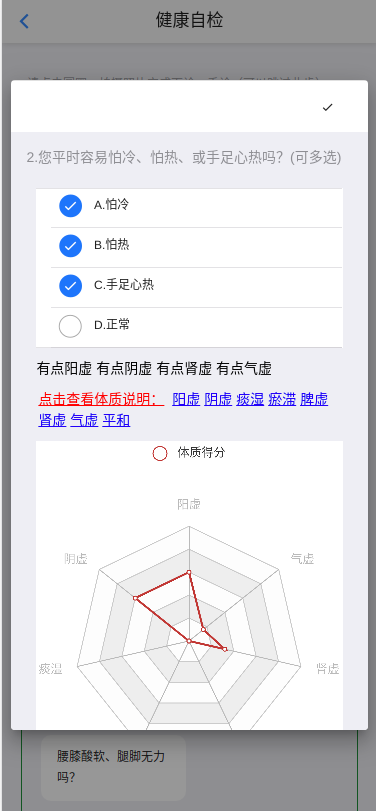
\includegraphics[height=10cm]{images/questions2.png}}
    \subfigure[解释体质术语]{
        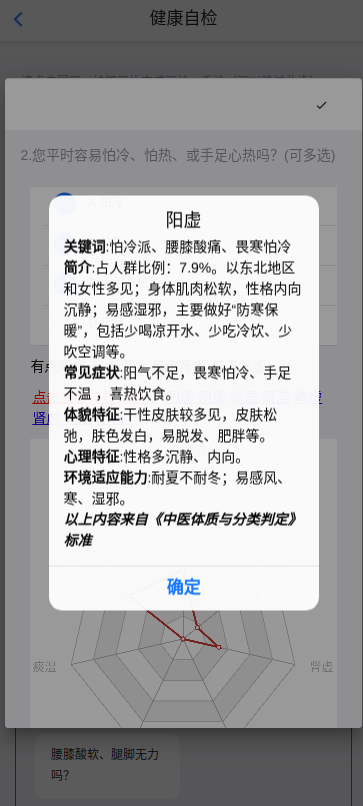
\includegraphics[height=10cm]{images/exp_phy.png}
    }
    \caption{问诊}
    \label{fig:questions}
\end{figure}

如图 \ref{fig:questions} 所示:

a) 普通用户,回答问诊问题之后,没有任何提示或者解释。

b) 透明类型的用户,在进行问诊过程中,可以立即看到每个答案对结果的印象,通过下方的雷达图显示了影响的体质倾向类型和具体的数值。
雷达图的更新是实时根据用户的选择进行更新的,提高了交互性。

c) 对中医术语中,各种体质的解释,对于体质内容的解释文字引用自 《中医体质分类研究》标准。



\subsection{诊断结果的透明性}
\begin{figure}[ht]
    \centering
    \subfigure[解释]{
        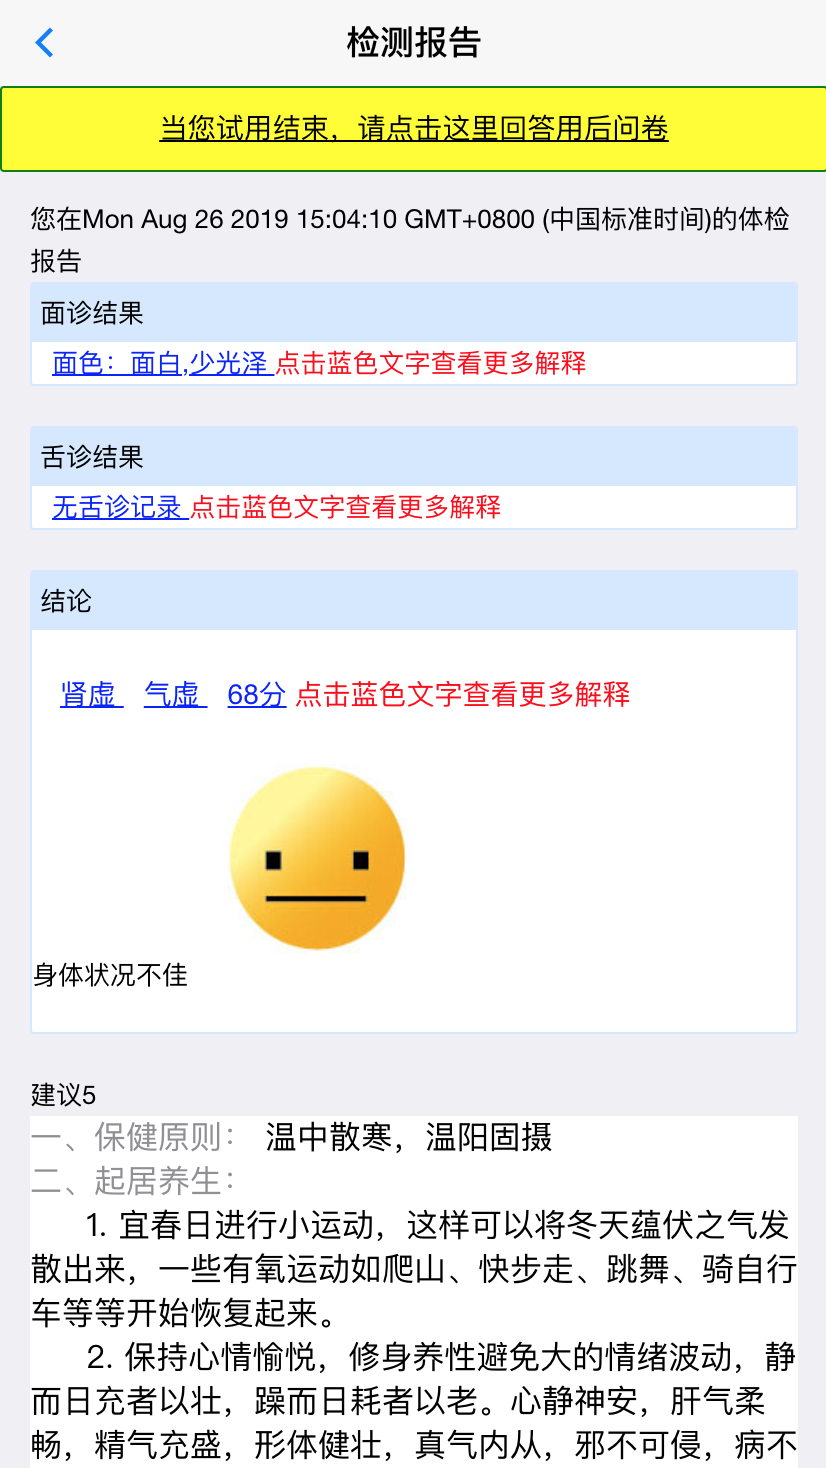
\includegraphics[height=10cm]{images/report3.png}
    }
    \subfigure[不解释]{
        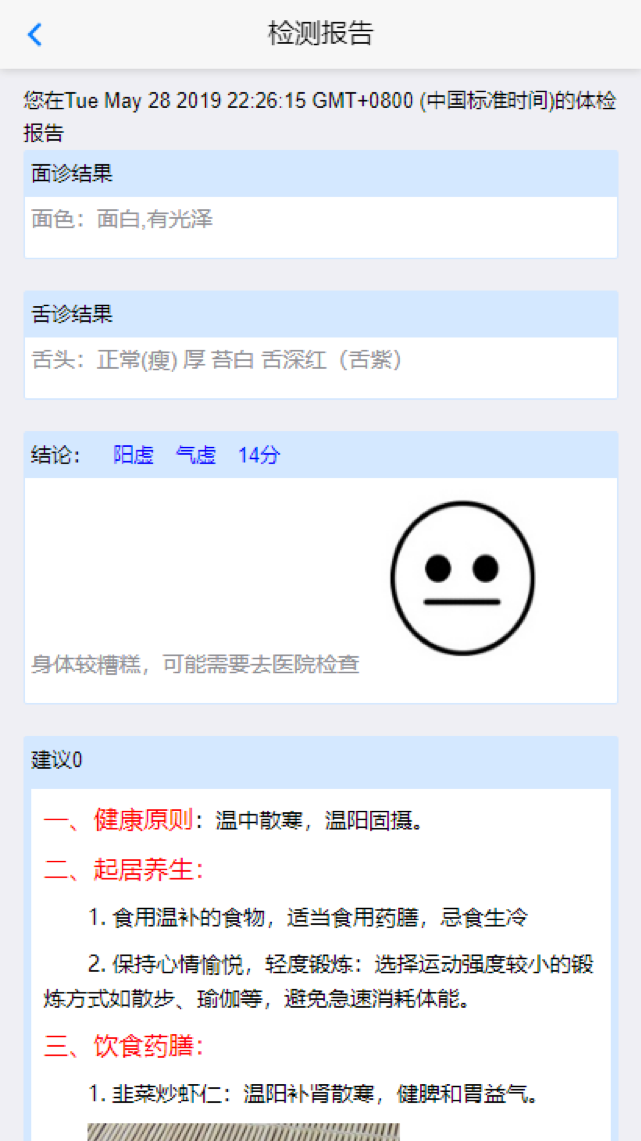
\includegraphics[height=10cm]{images/report.png}
    }
    \caption{诊断报告}
    \label{fig:my_label}
\end{figure}

普通用户在诊断结果页面,可以看到自己的健康分数和体质结果;透明用户可以点击诊断分数,了解这个分数是根据哪些指标,通过哪一个算法计算过来的。

可以点击查看的结果的解释有:面诊舌诊结果的解释,健康分数的解释,体质的解释。

\subsubsection{面诊舌诊结果的透明性}

\subsubsection{健康分数的透明性}
问诊结果的透明性主要是对用户透明诊断结果是如何计算出来的,以及那些问诊的问题对结果有影响,影响程度多少。

\begin{figure}[h]
    \centering
    \subfigure[相关问题]{
        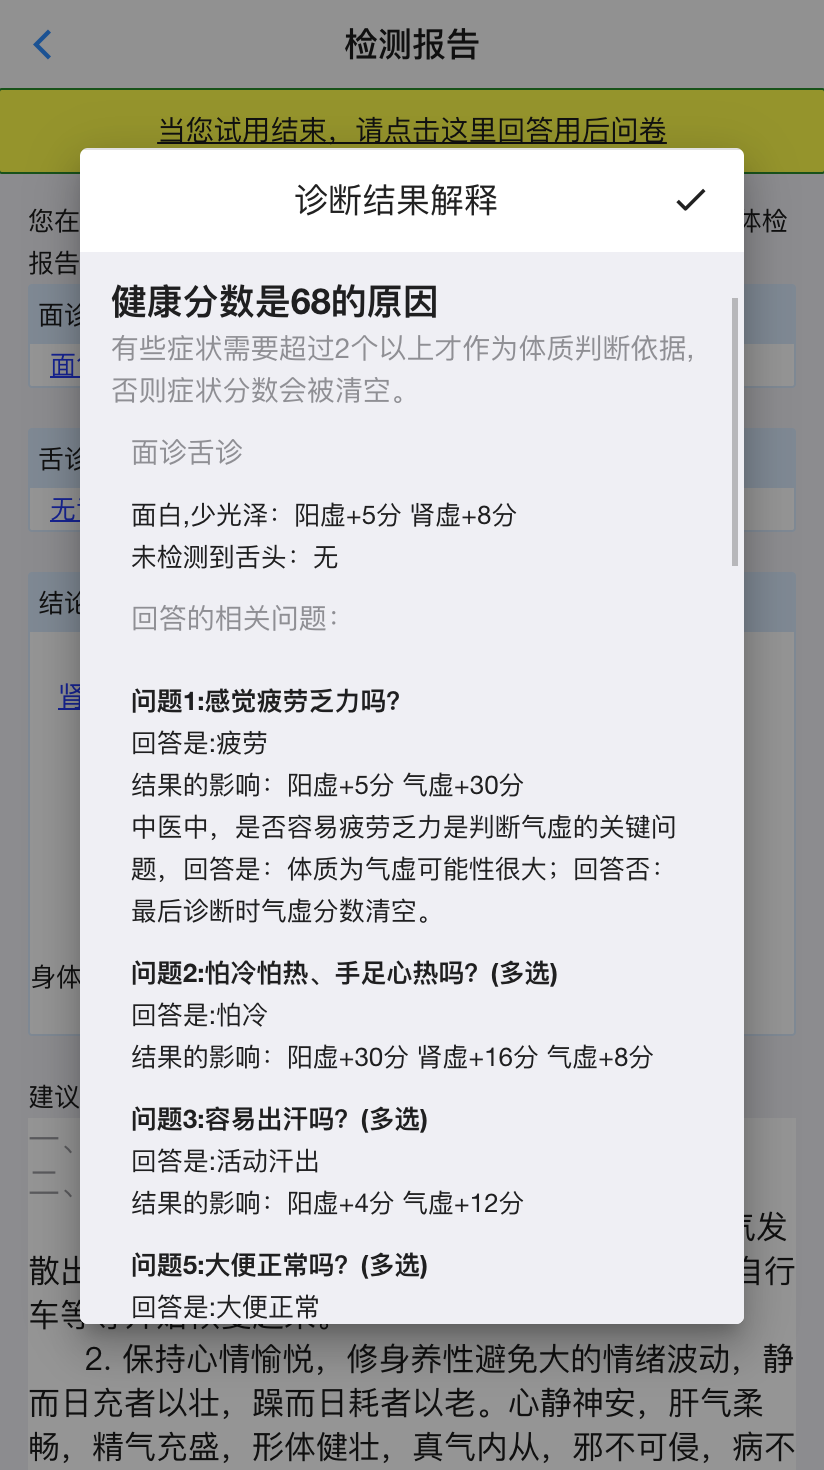
\includegraphics[height=7cm]{images/report7.png}
    }
    \subfigure[雷达图]{
        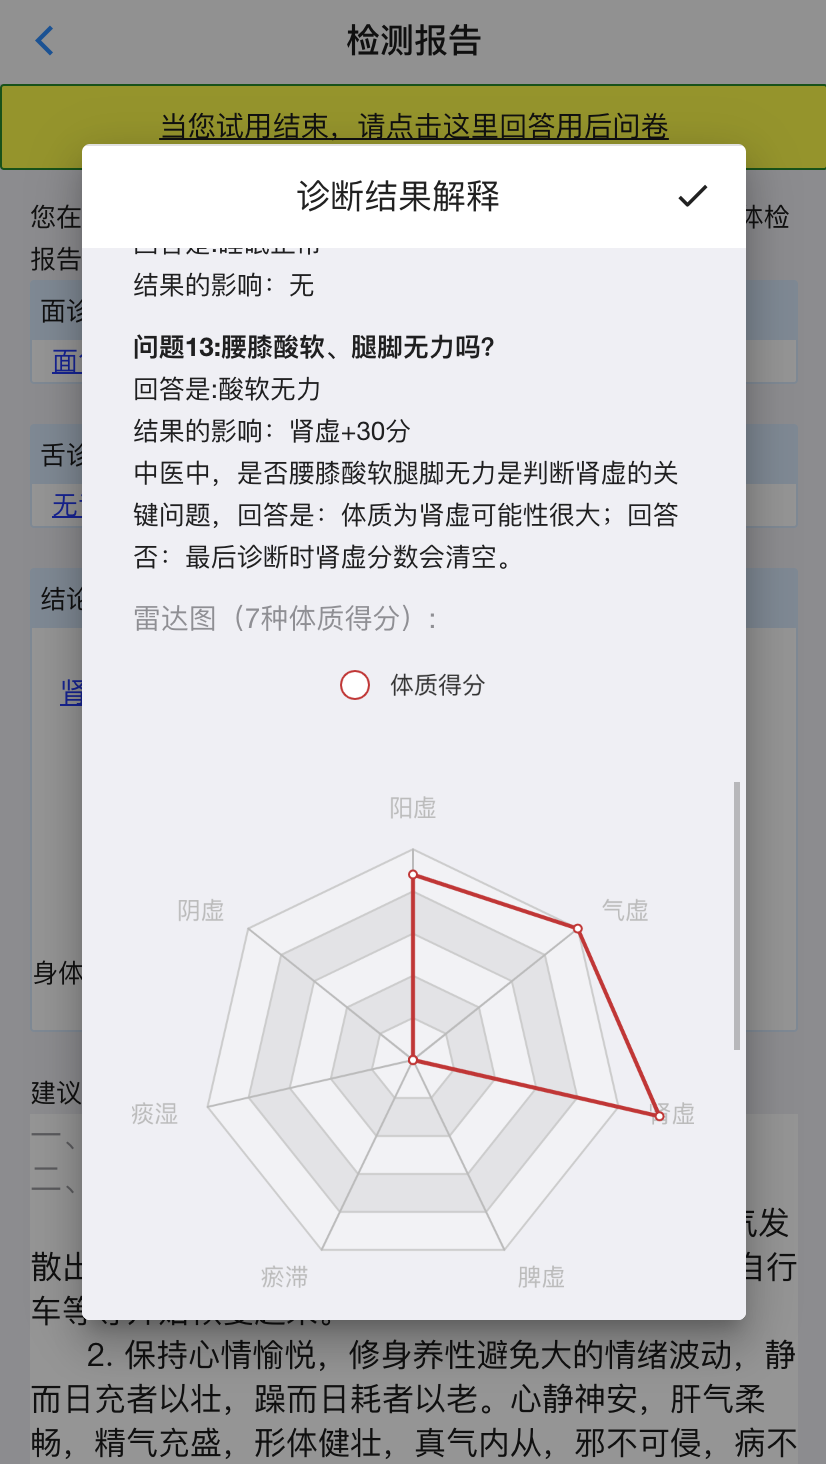
\includegraphics[height=7cm]{images/report8.png}
    }
    \subfigure[计算公式]{
        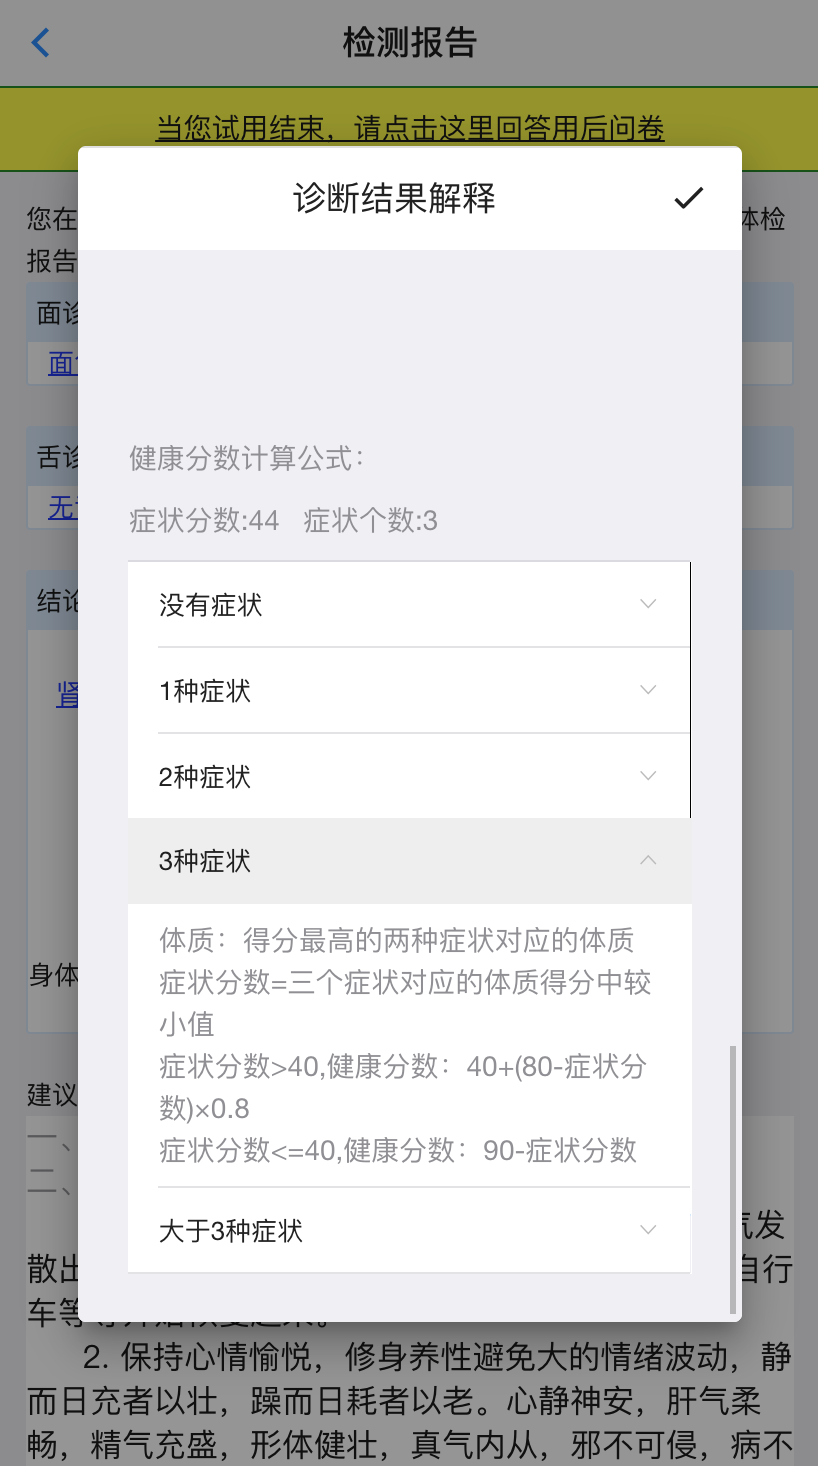
\includegraphics[height=7cm]{images/report9.png}
    }
    \caption{分数的解释}
    \label{fig:report_expalin_score}
\end{figure}

如图\ref{fig:report_expalin_score}所示,用户点击诊断页面的分数之后,弹窗里会显示分数相关的问题、雷达图和分数计算公式。

分数相关问题,展示了面诊舌诊对体质分数的影响和问诊对体质分数的影响,无影响的问题则不会显示。其中体质分数的变化分两种,一个是分数的累加,另一种是体质分数的清空。

雷达图对体质分数进行了汇总,给用户展示最终个人的体质倾向的结果。

根据诊断打分模型的内部算法,解释页面的计算公式一共有5种类别,我们使用选项卡的方式,将所有的打分计算公式全部透明给用户,并且默认打开当前计算公式的选项卡。

点击面诊结果,可以看到自己的面部舌部的对于整个诊断的影响。

点击体质分数,可以看到当次诊断中,面诊舌诊和用户自己回答的问题,哪些影响到了最后体质的判断。

\subsubsection{体质的解释}

\begin{figure}[ht]
    \centering
    \subfigure[面诊的解释]{
        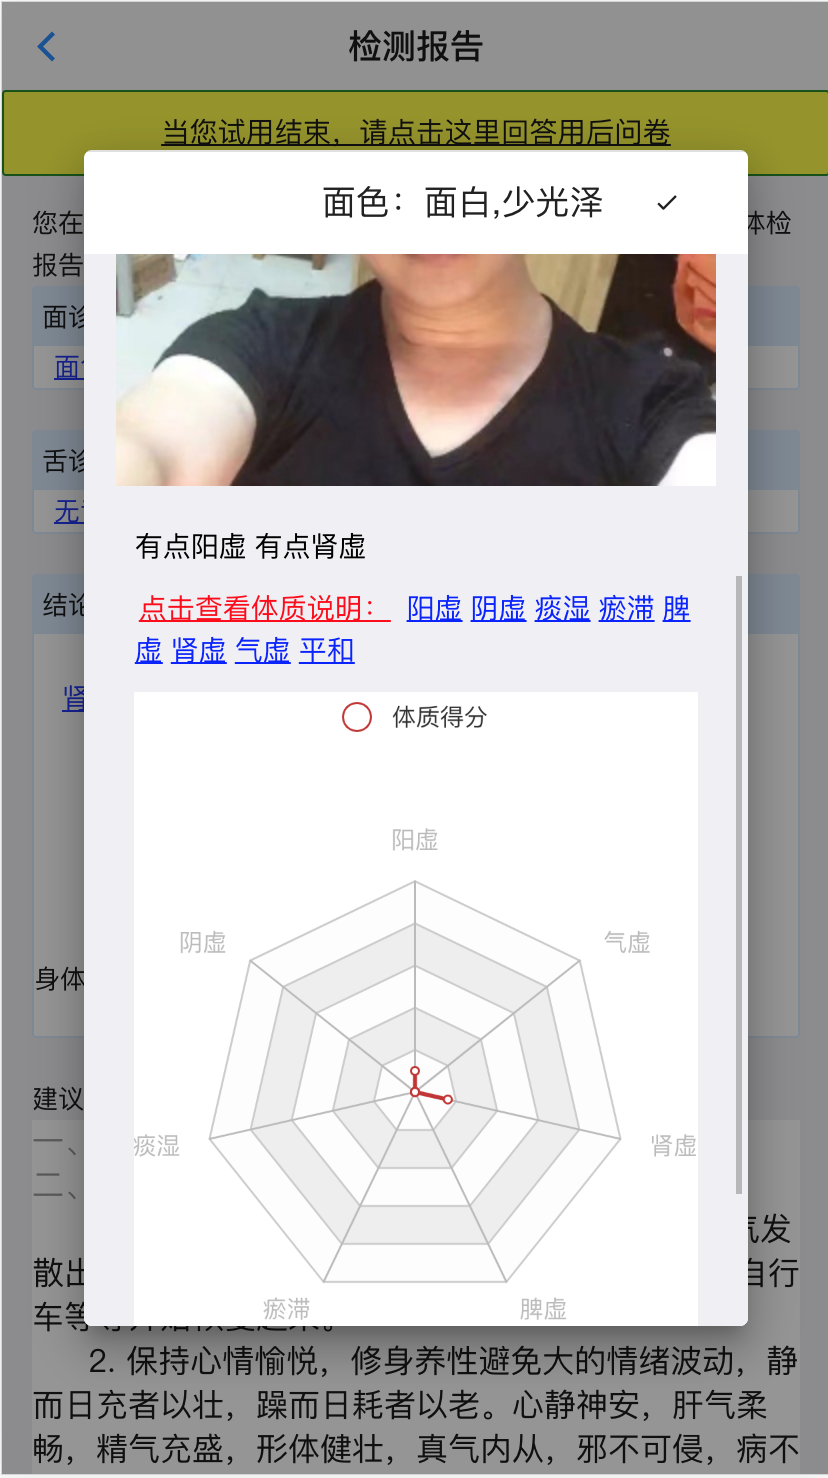
\includegraphics[height=7cm]{images/report4.png}
    }
    \subfigure[概念的解释]{
        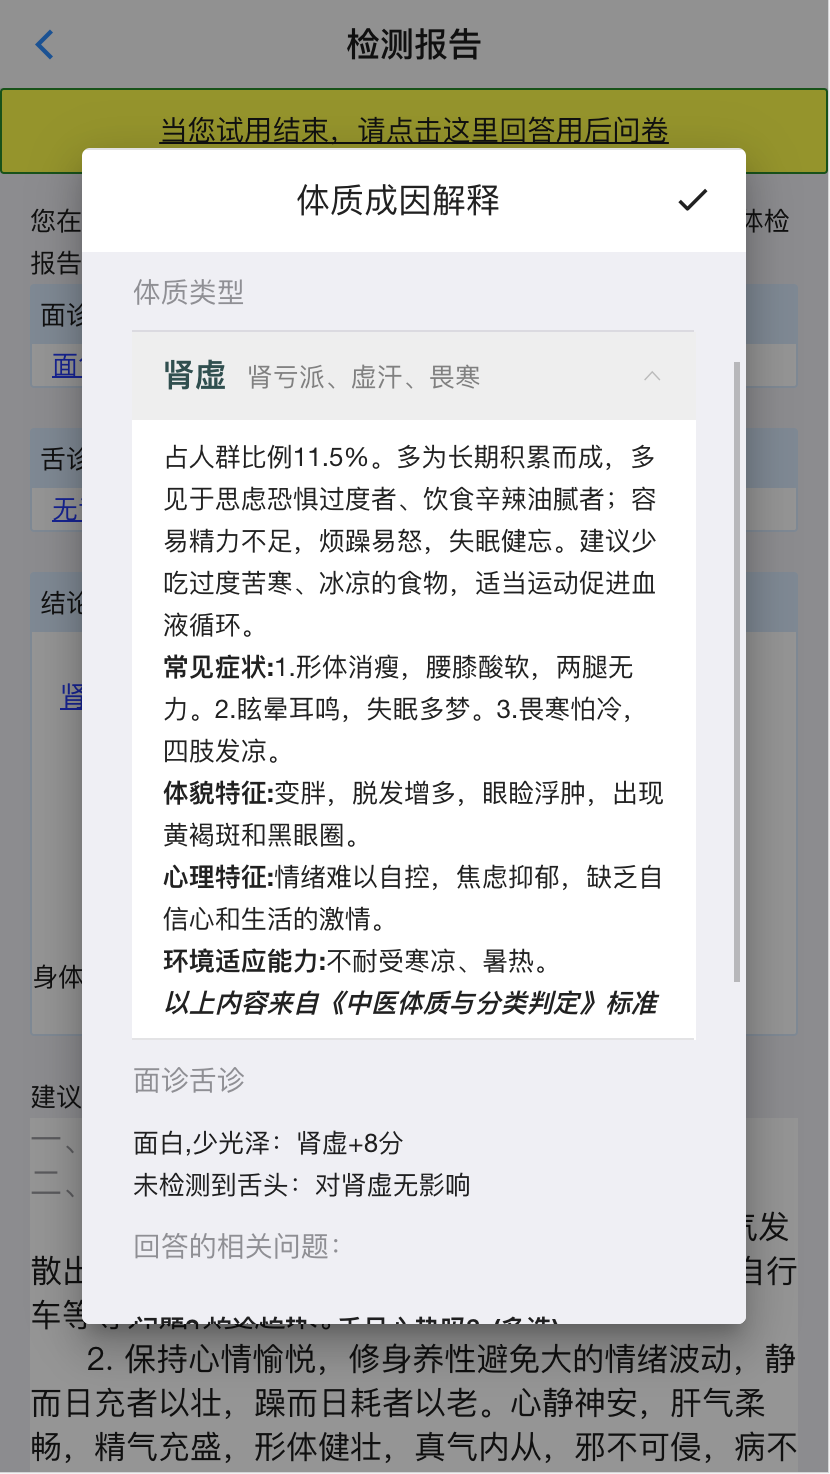
\includegraphics[height=7cm]{images/report5.png}
    }
    \subfigure[体质相关问题]{
        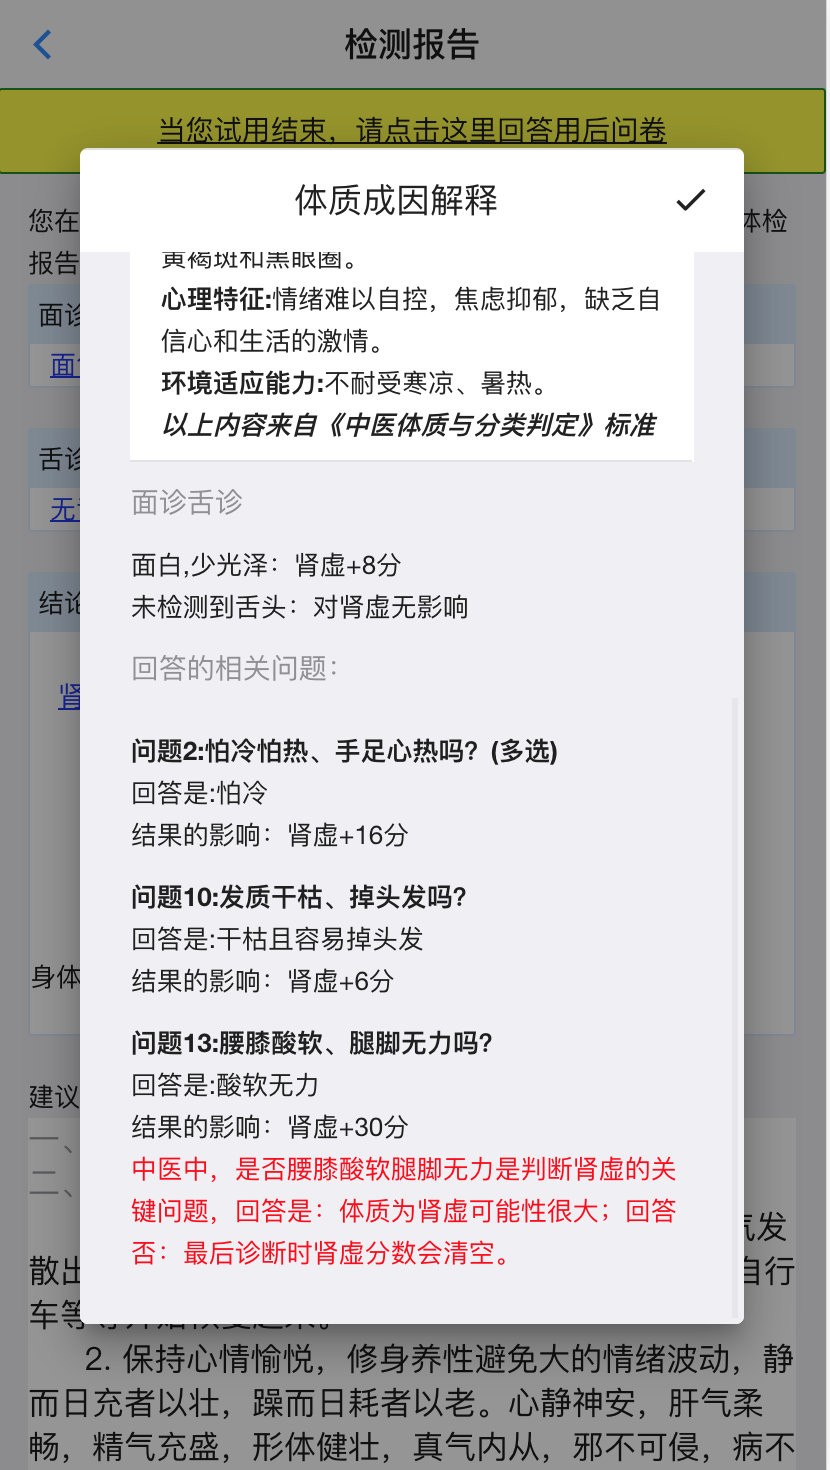
\includegraphics[height=7cm]{images/report6.png}
    }
    \caption{诊断结果的解释}
    \label{fig:report_explain_phy_1}
\end{figure}


\section{反馈调研}
在新系统完成之后,我们采访了16名用户。
在本次调研过程中,用户试用的是同时有新旧界面的版本,除了第一次介绍使用的时候,我们会让用户两个版本都是使用一下,后续不做限时。用户具体使用的时候可以根据自己的喜好选择。
经过回访,新版的界面达到了预期,大部分用户觉得使用起来更加地方便。
不过值得注意的是,也有少部分的用户喜欢旧版的将面诊,舌诊,问诊分开为三步进行的方式,因为这样比较符合日常生活的习惯。
